\documentclass{uofa-eng-assignment}
\usepackage{amsmath}
\usepackage{enumerate}% http://ctan.org/pkg/enumerate
\usepackage{lipsum}
\usepackage{hyperref}
\usepackage{amsmath, amsthm, amssymb, amsfonts, physics}
\usepackage{mathtools}
\usepackage{graphicx}
\usepackage{fdsymbol}

\hypersetup{
    colorlinks=true,
    linkcolor=blue,
    filecolor=magenta,
    urlcolor=cyan,
    pdftitle={Overleaf Example},
    pdfpagemode=FullScreen,
}

\graphicspath{ {./images/} }

\DeclareRobustCommand{\rchi}{{\mathpalette\irchi\relax}}
\newcommand{\infdiv}{D\infdivx}
\newcommand{\irchi}[2]{\raisebox{\depth}{$#1\chi$}} % inner command, used by \rchi
\newcommand\aug{\fboxsep=-\fboxrule\!\!\!\fbox{\strut}\!\!\!}
\newcommand*{\name}{\textbf{Luke Nguyen}}
\newcommand*{\id}{\textbf{D5850A}}
\newcommand*{\course}{Statistical Methods and Data Analysis (EN.625.603)}
\newcommand*{\assignment}{Problem Set 8}

\begin{document} \maketitle
%%%%%%%%%%%%%%%%%%%%%%%%%%%%%%%%%%%%%%%%%%%%%%%%%%%%%%%%%%%%%%%%%%%%%%%%%%%%%%%%%%%%%%%%%%%%%%%%%%%%    
\begin{enumerate}
    %%%%%%%%%%%%%%%%%%%%%%%%%%%%%%%%%%%%%%%%%%%%%%%%%%%%%%%%%%%%%%%%%%%%%%%%%%%%%%%%%%%%%%%%%%%%%%%%%%%%    
    %%%%%%%%%%%%%%%%%%%%%%%%%%%%%%%%%%%%%%%%%%%%%%%%%%%%%%%%%%%%%%%%%%%%%%%%%%%%%%%%%%%%%%%%%%%%%%%%%%%%    
    %%%%%%%%%%%%%%%%%%%%%%%%%%%%%%%%%%%%%%%%%%%%%%%%%%%%%%%%%%%%%%%%%%%%%%%%%%%%%%%%%%%%%%%%%%%%%%%%%%%%    
    %%%%%%%%%%%%%%%%%%%%%%%%%%%%%%%%%%%%%%%%%%%%%%%%%%%%%%%%%%%%%%%%%%%%%%%%%%%%%%%%%%%%%%%%%%%%%%%%%%%%    
    %%%%%%%%%%%%%%%%%%%%%%%%%%%%%%%%%%%%%%%%%%%%%%%%%%%%%%%%%%%%%%%%%%%%%%%%%%%%%%%%%%%%%%%%%%%%%%%%%%%%    
    \item[]
        \textbf{Question 11.2.1} \\
        \begin{table}[ht]
            \centering
            \begin{tabular}{ccc}
                \hline
                Observation No. & Chirps per Second (x) & Temperature (y) \\
                \hline
                1               & 20.0                  & 88.6            \\
                2               & 16.0                  & 71.6            \\
                3               & 19.8                  & 93.3            \\
                4               & 18.4                  & 84.3            \\
                5               & 17.1                  & 80.6            \\
                6               & 15.5                  & 75.2            \\
                7               & 14.7                  & 69.7            \\
                8               & 17.1                  & 82.0            \\
                9               & 15.4                  & 69.4            \\
                10              & 16.2                  & 83.3            \\
                11              & 15.0                  & 79.6            \\
                12              & 17.2                  & 82.6            \\
                13              & 16.0                  & 80.6            \\
                14              & 17.0                  & 83.5            \\
                15              & 14.4                  & 76.3            \\
                \hline
            \end{tabular}
        \end{table}
        \begin{align*}
            \sum_{i=1}^{15}x_1 & = 249.8 \qquad  & \sum_{i=1}^{15}x_i^2  & = 4200.56  \\
            \sum_{i=1}^{15}y_i & = 1200.6 \qquad & \sum_{i=1}^{15}x_iy_i & = 20127.47 \\
        \end{align*}
        \textbf{Solution} \\
        Using \textbf{Theorem 11.2.1}, we can calculate the slope as follows:
        \begin{align*}
            b     & = \frac{n\sum_{1}^{15}x_iy_i - \sum_{1}^{15}x_i\sum_{1}^{15}y_i}{n\sum_{1}^{15}x_i^2 - (\sum_{1}^{15}x_i)^2} \\
                  & = \frac{15(20127.47) - (249.8)(1200.6)}{15(4200.56) - (249.8)^2} = 3.291                                     \\
            a     & = \frac{\sum_{1}^{15}y_i}{n} - b\frac{\sum_{1}^{15}x_i}{n}                                                   \\
                  & = \frac{1200.6}{15} - (3.291)\frac{249.8}{15} = 25.234                                                       \\
            y(18) & = 25.234 + (3.291)(18) = 84.472
        \end{align*}
        \begin{figure}[h]
            \centering
            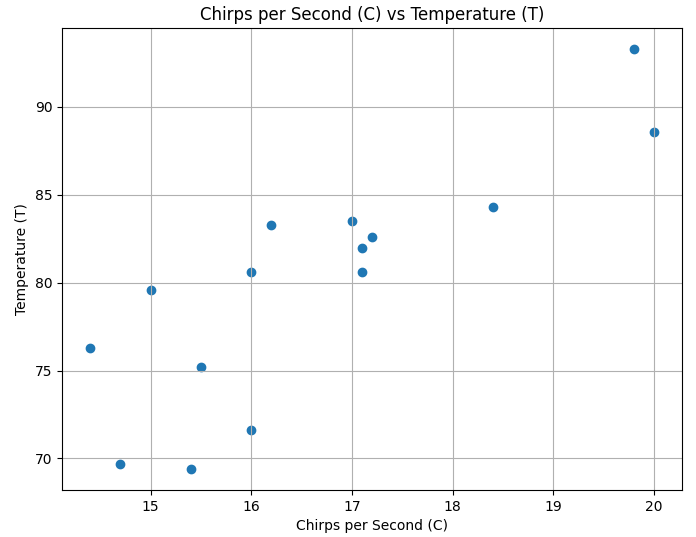
\includegraphics[width=0.6\textwidth]{11.2.1.png}
        \end{figure}
        %%%%%%%%%%%%%%%%%%%%%%%%%%%%%%%%%%%%%%%%%%%%%%%%%%%%%%%%%%%%%%%%%%%%%%%%%%%%%%%%%%%%%%%%%%%%%%%%%%%%    
        %%%%%%%%%%%%%%%%%%%%%%%%%%%%%%%%%%%%%%%%%%%%%%%%%%%%%%%%%%%%%%%%%%%%%%%%%%%%%%%%%%%%%%%%%%%%%%%%%%%%    
        %%%%%%%%%%%%%%%%%%%%%%%%%%%%%%%%%%%%%%%%%%%%%%%%%%%%%%%%%%%%%%%%%%%%%%%%%%%%%%%%%%%%%%%%%%%%%%%%%%%%    
        %%%%%%%%%%%%%%%%%%%%%%%%%%%%%%%%%%%%%%%%%%%%%%%%%%%%%%%%%%%%%%%%%%%%%%%%%%%%%%%%%%%%%%%%%%%%%%%%%%%%    
        %%%%%%%%%%%%%%%%%%%%%%%%%%%%%%%%%%%%%%%%%%%%%%%%%%%%%%%%%%%%%%%%%%%%%%%%%%%%%%%%%%%%%%%%%%%%%%%%%%%%    
    \item[]
        \textbf{Question 11.2.2} \\ \\
        \begin{table}[h]
            \centering
            \begin{tabular}{cc}
                \hline
                Age, x & Proof, y \\
                \hline
                0      & 104.6    \\
                0.5    & 104.1    \\
                1      & 104.4    \\
                2      & 105      \\
                3      & 106      \\
                4      & 106.8    \\
                5      & 107.7    \\
                6      & 108.7    \\
                7      & 110.6    \\
                8      & 112.1    \\
            \end{tabular}
        \end{table}
        \begin{align*}
            \sum_{i=1}^{10}x_i & = 36.5 \qquad & \sum_{i=1}^{10}x_i^2  & = 204.25  \\
            \sum_{i=1}^{10}y_i & = 1070 \qquad & \sum_{i=1}^{10}x_iy_i & = 3973.35 \\
        \end{align*}
        \textbf{Solution} \\
        Using \textbf{Theorem 11.2.1}, we can calculate the slope as follows:
        \begin{align*}
            b & = \frac{n\sum_{1}^{10}x_iy_i - \sum_{1}^{10}x_i\sum_{1}^{10}y_i}{n\sum_{1}^{10}x_i^2 - (\sum_{1}^{10}x_i)^2} \\
              & = \frac{10(3973.35) - (36.5)(1070)}{10(204.25) - (36.5)^2}                                                   \\
              & = 0.955                                                                                                      \\
            a & = \frac{\sum_{1}^{10}y_i}{n} - b\frac{\sum_{1}^{10}x_i}{n}                                                   \\
              & = \frac{1070}{10} - (0.955)\frac{36.5}{10}                                                                   \\
              & = 103.514                                                                                                    \\
            y & = 0.955x + 103.514
        \end{align*}
        \begin{figure}[h]
            \centering
            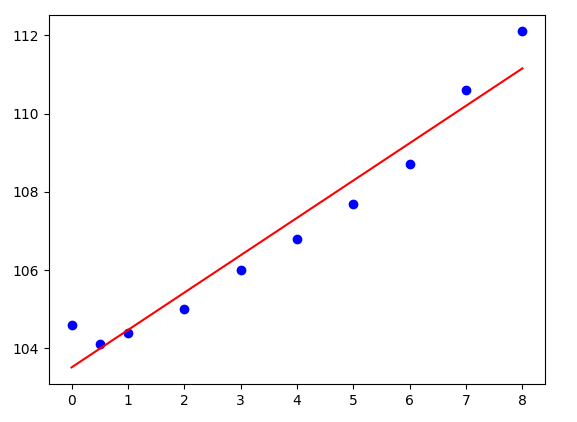
\includegraphics[width=0.6\textwidth]{11.2.2.png}
        \end{figure}
        %%%%%%%%%%%%%%%%%%%%%%%%%%%%%%%%%%%%%%%%%%%%%%%%%%%%%%%%%%%%%%%%%%%%%%%%%%%%%%%%%%%%%%%%%%%%%%%%%%%%    
        %%%%%%%%%%%%%%%%%%%%%%%%%%%%%%%%%%%%%%%%%%%%%%%%%%%%%%%%%%%%%%%%%%%%%%%%%%%%%%%%%%%%%%%%%%%%%%%%%%%%    
        %%%%%%%%%%%%%%%%%%%%%%%%%%%%%%%%%%%%%%%%%%%%%%%%%%%%%%%%%%%%%%%%%%%%%%%%%%%%%%%%%%%%%%%%%%%%%%%%%%%%    
        %%%%%%%%%%%%%%%%%%%%%%%%%%%%%%%%%%%%%%%%%%%%%%%%%%%%%%%%%%%%%%%%%%%%%%%%%%%%%%%%%%%%%%%%%%%%%%%%%%%%    
        %%%%%%%%%%%%%%%%%%%%%%%%%%%%%%%%%%%%%%%%%%%%%%%%%%%%%%%%%%%%%%%%%%%%%%%%%%%%%%%%%%%%%%%%%%%%%%%%%%%% 
    \item[]
        \textbf{Question 11.2.3} \\
        \begin{table}[h]
            \centering
            \begin{tabular}{c c}
                \hline
                Temperature, x & Parts Dissolved, y \\
                \hline
                0              & 66.7               \\
                4              & 71.0               \\
                10             & 76.3               \\
                15             & 80.6               \\
                21             & 85.7               \\
                29             & 92.9               \\
                36             & 99.4               \\
                51             & 113.6              \\
                68             & 125.1              \\
                \hline
            \end{tabular}
        \end{table}
        \begin{align*}
            \sum_{i=1}^{9}x_i & = 234 \qquad   & \sum_{i=1}^{9}x_i^2  & = 10144   \\
            \sum_{i=1}^{9}y_i & = 811.3 \qquad & \sum_{i=1}^{9}x_iy_i & = 24628.6 \\
        \end{align*}
        \textbf{Solution} \\
        Using \textbf{Theorem 11.2.1}, we can calculate the slope as follows:
        \begin{align*}
            b & = \frac{n\sum_{1}^{9}x_iy_i - \sum_{1}^{9}x_i\sum_{1}^{9}y_i}{n\sum_{1}^{9}x_i^2 - (\sum_{1}^{9}x_i)^2} \\
              & = \frac{9(24628.6) - (234)(811.3)}{9(10144) - (234)^2}                                                  \\
              & = 0.871                                                                                                 \\
            a & = \frac{\sum_{1}^{9}y_i}{n} - b\frac{\sum_{1}^{9}x_i}{n}                                                \\
              & = \frac{811.3}{9} - (0.871)\frac{234}{9}                                                                \\
              & = 67.498                                                                                                \\
            y & = 0.871x + 67.498
        \end{align*}
        Using \text{Definition 11.2.1}, we can calculate the residuals as follows:
        \begin{align*}
            r_i & = y_i - \hat{y}_i                       \\
                & = y_i - (0.871)x_i - 67.498             \\
            r_1 & = 66.7 - (0.871)(0) - 67.498 = -0.798   \\
            r_2 & = 71.0 - (0.871)(4) - 67.498 = 0.018    \\
            r_3 & = 76.3 - (0.871)(10) - 67.498 = 0.092   \\
            r_4 & = 80.6 - (0.871)(15) - 67.498 = 0.037   \\
            r_5 & = 85.7 - (0.871)(21) - 67.498 = -0.089  \\
            r_6 & = 92.9 - (0.871)(29) - 67.498 = 0.143   \\
            r_7 & = 99.4 - (0.871)(36) - 67.498 = 0.546   \\
            r_8 & = 113.6 - (0.871)(51) - 67.498 = 1.681  \\
            r_9 & = 125.1 - (0.871)(68) - 67.498 = -1.626 \\
        \end{align*}
        \begin{figure}[h]
            \centering
            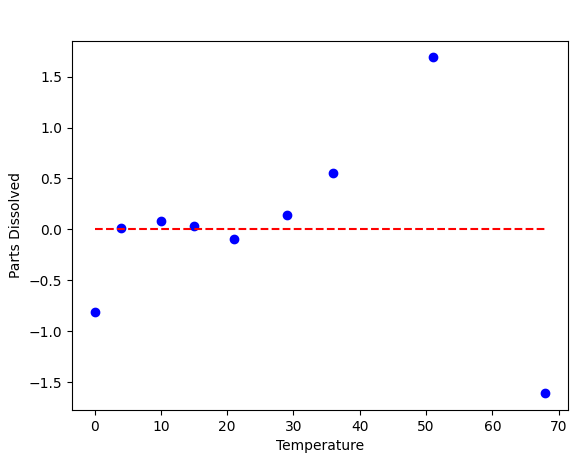
\includegraphics[width=0.5\textwidth]{11.2.3.png}
        \end{figure}
        %%%%%%%%%%%%%%%%%%%%%%%%%%%%%%%%%%%%%%%%%%%%%%%%%%%%%%%%%%%%%%%%%%%%%%%%%%%%%%%%%%%%%%%%%%%%%%%%%%%%    
        %%%%%%%%%%%%%%%%%%%%%%%%%%%%%%%%%%%%%%%%%%%%%%%%%%%%%%%%%%%%%%%%%%%%%%%%%%%%%%%%%%%%%%%%%%%%%%%%%%%%    
        %%%%%%%%%%%%%%%%%%%%%%%%%%%%%%%%%%%%%%%%%%%%%%%%%%%%%%%%%%%%%%%%%%%%%%%%%%%%%%%%%%%%%%%%%%%%%%%%%%%%    
        %%%%%%%%%%%%%%%%%%%%%%%%%%%%%%%%%%%%%%%%%%%%%%%%%%%%%%%%%%%%%%%%%%%%%%%%%%%%%%%%%%%%%%%%%%%%%%%%%%%%    
        %%%%%%%%%%%%%%%%%%%%%%%%%%%%%%%%%%%%%%%%%%%%%%%%%%%%%%%%%%%%%%%%%%%%%%%%%%%%%%%%%%%%%%%%%%%%%%%%%%%% 
    \item[]
        \textbf{Question 11.2.7}
        \begin{align*}
            \sum_{i=1}^{26}x_i & = 360 \qquad    & \sum_{i=1}^{26}x_i^2  & = 5365.08 \\
            \sum_{i=1}^{10}y_i & = 2256.6 \qquad & \sum_{i=1}^{26}x_iy_i & = 31402   \\
        \end{align*}
        \textbf{Solution} \\
        From \textbf{Theorem 11.2.1}, we can calculate the slope as follows:
        \begin{align*}
            b & = \frac{n\sum_{1}^{26}x_iy_i - \sum_{1}^{26}x_i\sum_{1}^{26}y_i}{n\sum_{1}^{26}x_i^2 - (\sum_{1}^{26}x_i)^2} \\
              & = \frac{26(31402) - (360)(2256.6)}{26(5365.08) - (360)^2}                                                    \\
              & = 0.412                                                                                                      \\
            a & = \frac{\sum_{1}^{26}y_i}{n} - b\frac{\sum_{1}^{26}x_i}{n}                                                   \\
              & = \frac{2256.6}{26} - (0.412)\frac{360}{26}                                                                  \\
              & = 81.088                                                                                                     \\
            y & = 0.412x + 81.088
        \end{align*}
        \begin{figure}[h]
            \centering
            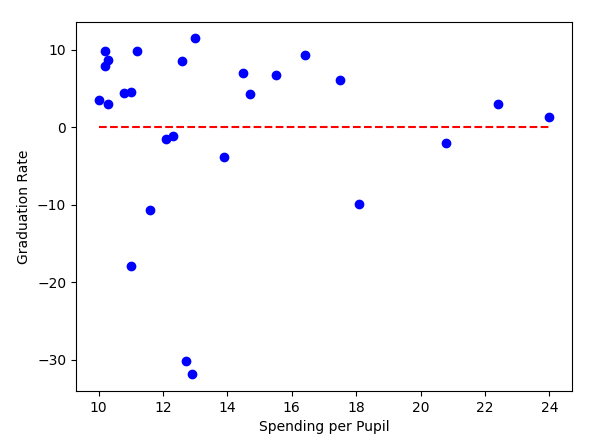
\includegraphics[width=0.54\textwidth]{11.2.7.png}
        \end{figure}
        %%%%%%%%%%%%%%%%%%%%%%%%%%%%%%%%%%%%%%%%%%%%%%%%%%%%%%%%%%%%%%%%%%%%%%%%%%%%%%%%%%%%%%%%%%%%%%%%%%%%    
        %%%%%%%%%%%%%%%%%%%%%%%%%%%%%%%%%%%%%%%%%%%%%%%%%%%%%%%%%%%%%%%%%%%%%%%%%%%%%%%%%%%%%%%%%%%%%%%%%%%%    
        %%%%%%%%%%%%%%%%%%%%%%%%%%%%%%%%%%%%%%%%%%%%%%%%%%%%%%%%%%%%%%%%%%%%%%%%%%%%%%%%%%%%%%%%%%%%%%%%%%%%    
        %%%%%%%%%%%%%%%%%%%%%%%%%%%%%%%%%%%%%%%%%%%%%%%%%%%%%%%%%%%%%%%%%%%%%%%%%%%%%%%%%%%%%%%%%%%%%%%%%%%%    
        %%%%%%%%%%%%%%%%%%%%%%%%%%%%%%%%%%%%%%%%%%%%%%%%%%%%%%%%%%%%%%%%%%%%%%%%%%%%%%%%%%%%%%%%%%%%%%%%%%%% 
    \item[]
        \textbf{Question 11.2.13} \\
        Prove that a least squares straight line must necessarily pass through the point $(\bar{x}, \bar{y})$. \\
        \textbf{Solution} \\
        Proof as follows:
        \begin{align*}
            \bar{y} & = \frac{\sum_{i=1}^{n}y_i}{n}                     \\
                    & = \frac{\sum_{i=1}^{n}(ax_i + b)}{n}              \\
                    & = \frac{a\sum_{i=1}^{n}x_i + b\sum_{i=1}^{n}1}{n} \\
                    & = \frac{a\sum_{i=1}^{n}x_i + bn}{n}               \\
                    & = a\bar{x} + b
        \end{align*}
        %%%%%%%%%%%%%%%%%%%%%%%%%%%%%%%%%%%%%%%%%%%%%%%%%%%%%%%%%%%%%%%%%%%%%%%%%%%%%%%%%%%%%%%%%%%%%%%%%%%%    
        %%%%%%%%%%%%%%%%%%%%%%%%%%%%%%%%%%%%%%%%%%%%%%%%%%%%%%%%%%%%%%%%%%%%%%%%%%%%%%%%%%%%%%%%%%%%%%%%%%%%    
        %%%%%%%%%%%%%%%%%%%%%%%%%%%%%%%%%%%%%%%%%%%%%%%%%%%%%%%%%%%%%%%%%%%%%%%%%%%%%%%%%%%%%%%%%%%%%%%%%%%%    
        %%%%%%%%%%%%%%%%%%%%%%%%%%%%%%%%%%%%%%%%%%%%%%%%%%%%%%%%%%%%%%%%%%%%%%%%%%%%%%%%%%%%%%%%%%%%%%%%%%%%    
        %%%%%%%%%%%%%%%%%%%%%%%%%%%%%%%%%%%%%%%%%%%%%%%%%%%%%%%%%%%%%%%%%%%%%%%%%%%%%%%%%%%%%%%%%%%%%%%%%%%% 
    \item[]
        \textbf{Question 11.2.14} \\
        In some regression situation, there are a priori reasons for assuming that
        the xy-relationship being approximated passes through the origin.
        If so, the equation to be fit to the $(x_i, y_i)'s$ has the form $y = bx$.
        Use the least squares criterio to show that the ``best`` slope in that case is given by
        \begin{align*}
            b = \frac{\sum_{i=1}^{n}x_iy_i}{\sum_{i=1}^{n}x_i^2}
        \end{align*}
        \textbf{Solution} \\
        Proof as follows:
        \begin{align*}
            \sum_{i=1}^{n}r_i^2                            & = \sum_{i=1}^{n}(y_i - bx_i)^2                                          \\
                                                           & = \sum_{i=1}^{n}(y_i^2 - 2bx_iy_i + b^2x_i^2)                           \\
                                                           & = \sum_{i=1}^{n}y_i^2 - 2b\sum_{i=1}^{n}x_iy_i + b^2\sum_{i=1}^{n}x_i^2 \\
            \frac{d}{db}\sum_{i=1}^{n}r_i^2                & = -2\sum_{i=1}^{n}x_iy_i + 2b\sum_{i=1}^{n}x_i^2                        \\
            \frac{d}{db}\sum_{i=1}^{n}r_i^2                & = 0                                                                     \\
            -2\sum_{i=1}^{n}x_iy_i + 2b\sum_{i=1}^{n}x_i^2 & = 0                                                                     \\
            2b\sum_{i=1}^{n}x_i^2                          & = 2\sum_{i=1}^{n}x_iy_i                                                 \\
            b                                              & = \frac{\sum_{i=1}^{n}x_iy_i}{\sum_{i=1}^{n}x_i^2}
        \end{align*}
        %%%%%%%%%%%%%%%%%%%%%%%%%%%%%%%%%%%%%%%%%%%%%%%%%%%%%%%%%%%%%%%%%%%%%%%%%%%%%%%%%%%%%%%%%%%%%%%%%%%%    
        %%%%%%%%%%%%%%%%%%%%%%%%%%%%%%%%%%%%%%%%%%%%%%%%%%%%%%%%%%%%%%%%%%%%%%%%%%%%%%%%%%%%%%%%%%%%%%%%%%%%    
        %%%%%%%%%%%%%%%%%%%%%%%%%%%%%%%%%%%%%%%%%%%%%%%%%%%%%%%%%%%%%%%%%%%%%%%%%%%%%%%%%%%%%%%%%%%%%%%%%%%%    
        %%%%%%%%%%%%%%%%%%%%%%%%%%%%%%%%%%%%%%%%%%%%%%%%%%%%%%%%%%%%%%%%%%%%%%%%%%%%%%%%%%%%%%%%%%%%%%%%%%%%    
        %%%%%%%%%%%%%%%%%%%%%%%%%%%%%%%%%%%%%%%%%%%%%%%%%%%%%%%%%%%%%%%%%%%%%%%%%%%%%%%%%%%%%%%%%%%%%%%%%%%% 
    \item[]
        \textbf{Question 11.3.2} \\
        The best straight line through the Massachusetts funding/graduation rate described in Question 11.2.7
        has the equation $y = 81.088 + 0.412x$, where $s = 11.78848$.
        \begin{itemize}
            \item [(a)] Construct a $95\%$ confident interval for $\beta_1$.
            \item [(b)] What does your answer to part (a) imply about the outcome of
                  testing $H_0: \beta_1 = 0$ versus $H_1: \beta_1 \neq 0$? at the $\alpha=0.05$ level of significance?
            \item [(c)] Graph teh data and superimpose the regressionline. How would you summarize these data,
                  and their implicatios, to a meeting of the state School Board?
        \end{itemize}
        \textbf{Solution} \\
        \begin{itemize}
            \item [(a)] From Question 11.2.7,
                  \begin{align*}
                      \sum_{i=1}^{26}x_i & = 360 \qquad      & \sum_{i=1}^{26}x_i^2  & = 5365.08 \\
                      \sum_{i=1}^{10}y_i & = 2256.6 \qquad   & \sum_{i=1}^{26}x_iy_i & = 31402   \\
                      \hat{\beta_0}      & = 81.088                                              \\
                      \hat{\beta_1}      & = 0.412                                               \\
                      y                  & = 0.412x + 81.088
                  \end{align*}
                  First, we can find the degrees of freedom and $t$ random variable as follows
                  \begin{align*}
                      df                & = n - 2         \\
                                        & = 24            \\
                      t_{\alpha/2, n-2} & = t_{0.025, 24} \\
                                        & = 2.064
                  \end{align*}
                  Using \textbf{Theorem 11.3.6}, we can calculate the $95\%$ confidence interval as follows:
                  \begin{align*}
                       & = \hat{\beta_1} \pm t_{\alpha/2, n-2}\frac{s}{\sqrt{\sum_{i=1}^{n}(x_i - \bar{x})^2}} \\
                       & = 0.412 \pm 2.064\frac{11.78848}{\sqrt{380.46}}                                       \\
                       & = (-0.835, 1.659)
                  \end{align*}
            \item [(b)] Since $0$ is in the confidence interval, we fail to reject the null hypothesis.
            \item [(c)] As we shown in the graph above in the solution to question 11.2.7, there is no strong linear relationship between
                  the funding and graduation rate. The regression line is not a good fit for the data.
        \end{itemize}
        %%%%%%%%%%%%%%%%%%%%%%%%%%%%%%%%%%%%%%%%%%%%%%%%%%%%%%%%%%%%%%%%%%%%%%%%%%%%%%%%%%%%%%%%%%%%%%%%%%%%    
        %%%%%%%%%%%%%%%%%%%%%%%%%%%%%%%%%%%%%%%%%%%%%%%%%%%%%%%%%%%%%%%%%%%%%%%%%%%%%%%%%%%%%%%%%%%%%%%%%%%%    
        %%%%%%%%%%%%%%%%%%%%%%%%%%%%%%%%%%%%%%%%%%%%%%%%%%%%%%%%%%%%%%%%%%%%%%%%%%%%%%%%%%%%%%%%%%%%%%%%%%%%    
        %%%%%%%%%%%%%%%%%%%%%%%%%%%%%%%%%%%%%%%%%%%%%%%%%%%%%%%%%%%%%%%%%%%%%%%%%%%%%%%%%%%%%%%%%%%%%%%%%%%%    
        %%%%%%%%%%%%%%%%%%%%%%%%%%%%%%%%%%%%%%%%%%%%%%%%%%%%%%%%%%%%%%%%%%%%%%%%%%%%%%%%%%%%%%%%%%%%%%%%%%%% 
    \item[]
        \textbf{Question 11.3.14} \\
        Construct a $90\%$ confidence interval for $\sigma^2$ in the cigarette-consumption/CHD mortality data
        given in Case Study 11.3.1. \\
        \textbf{Solution} \\
        From Case Study 11.3.1, we have
        \begin{align*}
            \beta_0 = 15.771 \\
            \beta_1 = 0.0601 \\
            s^2 & = 2181.588
        \end{align*}
        First we can find the degrees of freedom and $\chi^2$ random variable as follows
        \begin{align*}
            df                       & = n - 2             \\
                                     & = 19                \\
            \chi^2_{\alpha/2, n-2}   & = \chi^2_{0.05, 19} \\
                                     & = 10.117            \\
            \chi^2_{1-\alpha/2, n-2} & = \chi^2_{0.95, 19} \\
                                     & = 30.144
        \end{align*}
        Using \textbf{drawing interferences about $\sigma^2$}, we can calculate the $90\%$ confidence interval as follows
        \begin{align*}
             & = \left(\frac{(n-2)s^2}{\chi^2_{1-\alpha/2, n-2}}, \frac{(n-2)s^2}{\chi^2_{\alpha/2, n-2}}\right) \\
             & = (1375.072, 4097.081)
        \end{align*}
        %%%%%%%%%%%%%%%%%%%%%%%%%%%%%%%%%%%%%%%%%%%%%%%%%%%%%%%%%%%%%%%%%%%%%%%%%%%%%%%%%%%%%%%%%%%%%%%%%%%%    
        %%%%%%%%%%%%%%%%%%%%%%%%%%%%%%%%%%%%%%%%%%%%%%%%%%%%%%%%%%%%%%%%%%%%%%%%%%%%%%%%%%%%%%%%%%%%%%%%%%%%    
        %%%%%%%%%%%%%%%%%%%%%%%%%%%%%%%%%%%%%%%%%%%%%%%%%%%%%%%%%%%%%%%%%%%%%%%%%%%%%%%%%%%%%%%%%%%%%%%%%%%%    
        %%%%%%%%%%%%%%%%%%%%%%%%%%%%%%%%%%%%%%%%%%%%%%%%%%%%%%%%%%%%%%%%%%%%%%%%%%%%%%%%%%%%%%%%%%%%%%%%%%%%    
        %%%%%%%%%%%%%%%%%%%%%%%%%%%%%%%%%%%%%%%%%%%%%%%%%%%%%%%%%%%%%%%%%%%%%%%%%%%%%%%%%%%%%%%%%%%%%%%%%%%% 
    \item[]
        \textbf{Question 11.3.16}
        \begin{align*}
            y       & = -0.104 + 0.988x \\
            \beta_0 & = -0.104          \\
            \beta_1 & = 0.988           \\
        \end{align*}
        \textbf{Solution}
        \begin{itemize}
            \item [(a)]
                  For $x = 14$,
                  \begin{align*}
                      \hat{y} & = -0.104 + 0.988(14) \\
                              & = 13.728
                  \end{align*}
                  We  can calculate degress of freedom and $t$ random variable as follows
                  \begin{align*}
                      df                & = 18 - 2        \\
                                        & = 16            \\
                      t_{\alpha/2, n-2} & = t_{0.025, 16} \\
                                        & = 2.1199
                  \end{align*}
                  Applying \textbf{Theorem 11.3.8}, we can calculate the $95\%$ confidence interval as follows
                  \begin{align*}
                      w           & = t_{\alpha/2, n-2}\sqrt{s^2\left(\frac{1}{n} + \frac{(x - \bar{x})^2}{\sum_{i=1}^{n}(x_i - \bar{x})^2}\right)} \\
                      w           & = 0.109                                                                                                         \\
                      CI_{95\%} = & = 13.728 \pm 0.109                                                                                              \\
                                  & = (13.619, 13.837)
                  \end{align*}
            \item [(b)]
                  Using the result from (a), we can construct the $CI_{95\%}$ prediction interval as follows
                  \begin{align*}
                      w           & = t_{\alpha/2, n-2}\sqrt{s^2\left(1 + \frac{1}{n} + \frac{(x - \bar{x})^2}{\sum_{i=1}^{n}(x_i - \bar{x})^2}\right)} \\
                      w           & = 0.442                                                                                                             \\
                      CI_{95\%} = & = 13.728 \pm 0.442                                                                                                  \\
                                  & = (13.286, 14.170)
                  \end{align*}
        \end{itemize}
        %%%%%%%%%%%%%%%%%%%%%%%%%%%%%%%%%%%%%%%%%%%%%%%%%%%%%%%%%%%%%%%%%%%%%%%%%%%%%%%%%%%%%%%%%%%%%%%%%%%%    
        %%%%%%%%%%%%%%%%%%%%%%%%%%%%%%%%%%%%%%%%%%%%%%%%%%%%%%%%%%%%%%%%%%%%%%%%%%%%%%%%%%%%%%%%%%%%%%%%%%%%    
        %%%%%%%%%%%%%%%%%%%%%%%%%%%%%%%%%%%%%%%%%%%%%%%%%%%%%%%%%%%%%%%%%%%%%%%%%%%%%%%%%%%%%%%%%%%%%%%%%%%%    
        %%%%%%%%%%%%%%%%%%%%%%%%%%%%%%%%%%%%%%%%%%%%%%%%%%%%%%%%%%%%%%%%%%%%%%%%%%%%%%%%%%%%%%%%%%%%%%%%%%%%    
        %%%%%%%%%%%%%%%%%%%%%%%%%%%%%%%%%%%%%%%%%%%%%%%%%%%%%%%%%%%%%%%%%%%%%%%%%%%%%%%%%%%%%%%%%%%%%%%%%%%%   
    \item[]
        \textbf{Question 11.3.17}
        Construct a $95\%$ confidence interval $E(Y|2.750)$ using the connecting rod data given in Case Study 11.2.1.
        \begin{align*}
            \sum_{i=1}^{25}x_i    & = 66.075 \qquad \sum_{i=1}^{25}x_i^2 = 174.672925 \\
            \sum_{i=1}^{25}y_i    & = 50.12 \qquad \sum_{i=1}^{25}y_i^2 = 100.49865   \\
            \sum_{i=1}^{25}x_iy_i & = 132.490725                                      \\
            b                     & = 0.642 \qquad a = 0.308
        \end{align*}
        \textbf{Solution} \\
        For $x = 2.750$,
        \begin{align*}
            \hat{y} & = 0.308 + 0.642(2.750) \\
                    & = 2.0735
        \end{align*}
        We can calculate the degrees of freedom and $t$ random variable as follows
        \begin{align*}
            df                & = 25 - 2        \\
                              & = 23            \\
            t_{\alpha/2, n-2} & = t_{0.025, 23} \\
                              & = 2.069
        \end{align*}
        We can calculate sample variance as follows
        \begin{align*}
            s^2 & = \frac{1}{n-2}\left[\sum_{i=1}^{n}y_i^2 - b\sum_{i=1}^{n}x_iy_i\right] \\
                & = 0.0001149
        \end{align*}
        We can calculate the $95\%$ confidence interval as follows
        \begin{align*}
            w           & = t_{\alpha/2, n-2}\sqrt{s^2\left(\frac{1}{n} + \frac{(x - \bar{x})^2}{\sum_{i=1}^{n}(x_i - \bar{x})^2}\right)} \\
            w           & = 0.013                                                                                                         \\
            CI_{95\%} = & = 2.074 \pm 0.013                                                                                               \\
                        & = (2.061, 2.087)
        \end{align*}
        %%%%%%%%%%%%%%%%%%%%%%%%%%%%%%%%%%%%%%%%%%%%%%%%%%%%%%%%%%%%%%%%%%%%%%%%%%%%%%%%%%%%%%%%%%%%%%%%%%%%    
        %%%%%%%%%%%%%%%%%%%%%%%%%%%%%%%%%%%%%%%%%%%%%%%%%%%%%%%%%%%%%%%%%%%%%%%%%%%%%%%%%%%%%%%%%%%%%%%%%%%%    
        %%%%%%%%%%%%%%%%%%%%%%%%%%%%%%%%%%%%%%%%%%%%%%%%%%%%%%%%%%%%%%%%%%%%%%%%%%%%%%%%%%%%%%%%%%%%%%%%%%%%    
        %%%%%%%%%%%%%%%%%%%%%%%%%%%%%%%%%%%%%%%%%%%%%%%%%%%%%%%%%%%%%%%%%%%%%%%%%%%%%%%%%%%%%%%%%%%%%%%%%%%%    
        %%%%%%%%%%%%%%%%%%%%%%%%%%%%%%%%%%%%%%%%%%%%%%%%%%%%%%%%%%%%%%%%%%%%%%%%%%%%%%%%%%%%%%%%%%%%%%%%%%%%      
    \item[]
        \textbf{Question 11.4.12} \\
        \begin{align*}
            \sum_{i=1}^{30}x_i    & = 1300.69 \qquad \sum_{i=1}^{30}y_i = 323        \\
            \sum_{i=1}^{30}x_i^2  & = 86754.6939 \qquad \sum_{i=1}^{30}y_i^2 = 11881 \\
            \sum_{i=1}^{30}x_iy_i & = 7807.36
        \end{align*}
        \textbf{Solution} \\
        Using \textbf{sample correlation coefficient} formula, we can calculate the sample correlation coefficient as follows
        \begin{align*}
            R & = \frac{n\sum_{i=1}^{n}X_iY_i - \sum_{i=1}^{n}X_i\sum_{i=1}^{n}Y_i}{\sqrt{n\sum_{i=1}^{n}X_i^2 - \left(\sum_{i=1}^{n}X_i\right)^2}\sqrt{n\sum_{i=1}^{n}Y_i^2 - \left(\sum_{i=1}^{n}Y_i\right)^2}} \\
              & = \frac{30(7807.36) - (1300.69)(323)}{\sqrt{30(86754.6939) - (1300.69)^2}\sqrt{30(11881) - (323)^2}}                                                                                              \\
              & = -0.388
        \end{align*}
        It suggests that increasing bonus is associated with decreasing performance.
        %%%%%%%%%%%%%%%%%%%%%%%%%%%%%%%%%%%%%%%%%%%%%%%%%%%%%%%%%%%%%%%%%%%%%%%%%%%%%%%%%%%%%%%%%%%%%%%%%%%%    
        %%%%%%%%%%%%%%%%%%%%%%%%%%%%%%%%%%%%%%%%%%%%%%%%%%%%%%%%%%%%%%%%%%%%%%%%%%%%%%%%%%%%%%%%%%%%%%%%%%%%    
        %%%%%%%%%%%%%%%%%%%%%%%%%%%%%%%%%%%%%%%%%%%%%%%%%%%%%%%%%%%%%%%%%%%%%%%%%%%%%%%%%%%%%%%%%%%%%%%%%%%%    
        %%%%%%%%%%%%%%%%%%%%%%%%%%%%%%%%%%%%%%%%%%%%%%%%%%%%%%%%%%%%%%%%%%%%%%%%%%%%%%%%%%%%%%%%%%%%%%%%%%%%    
        %%%%%%%%%%%%%%%%%%%%%%%%%%%%%%%%%%%%%%%%%%%%%%%%%%%%%%%%%%%%%%%%%%%%%%%%%%%%%%%%%%%%%%%%%%%%%%%%%%%% 
\end{enumerate}
%%%%%%%%%%%%%%%%%%%%%%%%%%%%%%%%%%%%%%%%%%%%%%%%%%%%%%%%%%%%%%%%%%%%%%%%%%%%%%%%%%%%%%%%%%%%%%%%%%%%    
\end{document}